% F13: Section 5.4: historical grasping/PRM study, if retained. Read figures/FIGURE_GUIDE.md before reuse.
\begin{figure}[tbp]
  \centering
  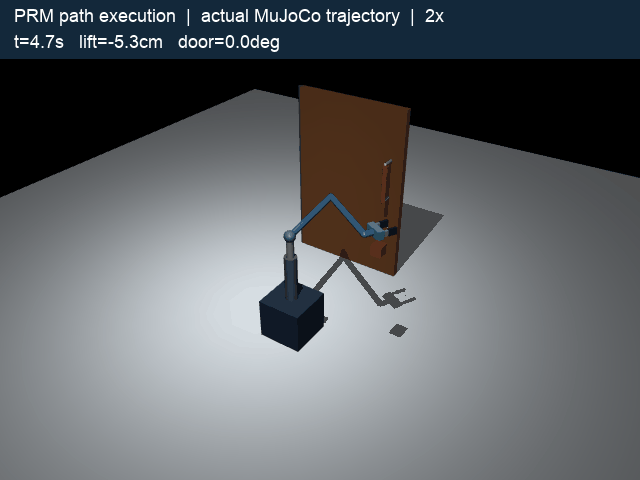
\includegraphics[width=.48\linewidth]{figures/optional_prm/F13_prm_detour_1.png}
  \hfill
  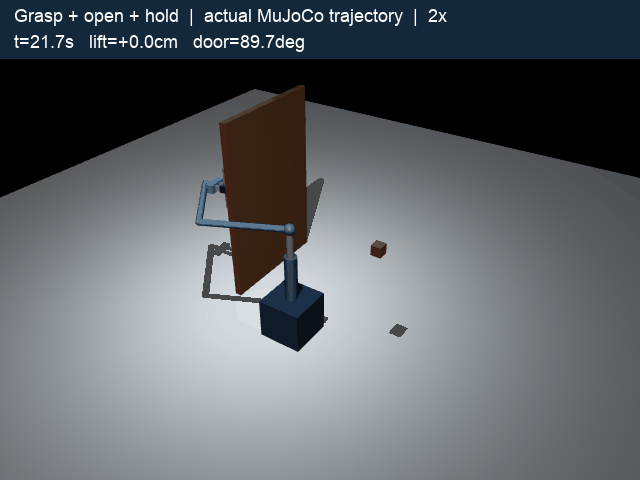
\includegraphics[width=.48\linewidth]{figures/optional_prm/F13_prm_detour_2.png}
  \hfill
  \caption{Independent PRM demonstration. Left: preparation follows a roadmap path around a configured obstacle (500 valid sampled nodes, five path points). Right: the subsequent physical grasp-and-open trial succeeds. This illustrative detour is separate from the 1512-record PRM training dataset, whose preparations all used direct paths, and from the mobile RRT planner.}
  \label{fig:prm_detour}
\end{figure}
